\section{Aufbau und Durchführung}
\label{sec:AundD}

\subsection{Aufbau}
\label{sec:Aufbau}

Der Aufbau des Experiments ist in Abbildung \ref{fig:aufbau} dargestellt. Für den Versuch wird ein Dewar-Gefäß verwendet, in dem im Laufe des Experiments flüssiger Stickstoff gefüllt wird, damit der
Rezipient gekühlt werden kann. Im Rezipienten befindet sich die zu untersuchende Kupferprobe. In der Kupferprobe befindet sich eine Heizwicklung, womit die Probe erhitzt werden kann. Um die Kupferprobe befindet sich noch ein Kupfer-Zylinder, der ebenfalls über eine Heizwicklung verfügt. Beide Heizwicklungen können jeweils getrennt voneinander über eine Stromversorgung bzw. ein Konstantstromgerät mit elektrischer Energie versorgt werden. Zusätzlich befindet sich im Zylinder und an der Probe jeweils ein PT-100 Messwiderstand über den mit Hilfe eines Ohmmeters der Widerstand gemessen werden kann. Der Widerstand varriert mit der Temperatur, dadurch kann aus dem Widerstand auf die Temperatur geschlossen werden. Außerdem ist der Rezipient noch mit einer Vakuumpumpe und einer Heliumflasche inklusive Absperrhahn und Reduzierventil verbunden. 

\begin{figure}[H]
    \centering
    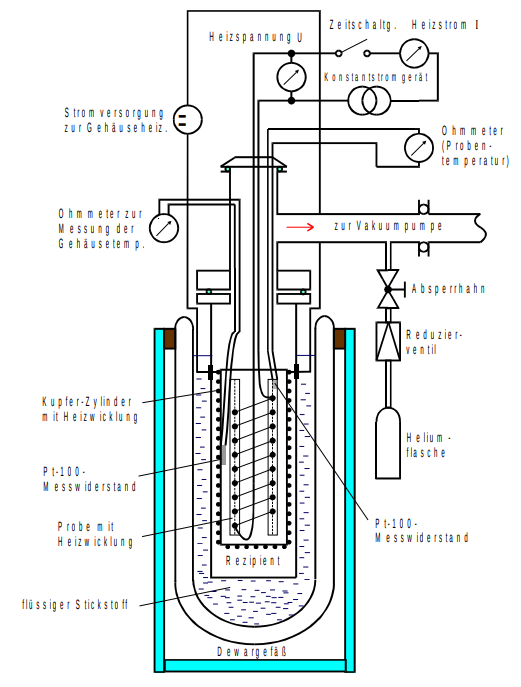
\includegraphics[width=0.8\textwidth]{build/Aufbau.PNG}
    \caption{Schematischer Aufbau des Versuchs %Quelle einfügen}
    \label{fig:aufbau}
\end{figure}

\subsection{Durchführung}
\label{sec:Durchfuehrung}

Zu Beginn wird der Rezipient mit Hilfe der Vakuumpumpe evakuiert. Nach der Evakuierung wird der Rezipient mit Helium gefüllt, damit beim Abkühlen ein möglichst großer Wärmefluss stattfinden kann, denn Helium hat eine hohe thermische Leitfähigkeit. Anschließend wird das Dewar-Gefäß mit flüssigen Stickstoff gefüllt und der Rezipient wird bis zu einer Temperatur von $80 \, \mathrm{K}$ abgekühlt. Wenn sowohl die Probe als auch der Zylinder die gewünschte Temperatur erreicht haben, wird der Rezipient wieder evakuiert, damit möglichst keine Konvektion mehr stattfinden kann und die Messung kann beginnen. Dazu wird die Probe über ein Konstantstromgerät beheizt und die Zeitmessung wird gestartet. Damit keine Wärmeverluste durch Konduktion von der Probe zum Zylinder stattfinden, sollte die Temperatur zwischen Zylinder und Probe immer identisch gehalten werden. Dafür muss die Leistung für die Heizwicklung vom Zylinder so varriert werden, dass die beiden Temperaturen sich nicht unterscheiden. Also sollte die Stromversorgung zur Gehäuseheizung stetig angepasst werden. Im Kontext der Durchführung bedeutet dies, dass der Widerstand der beiden Messwiderstände identisch gehalten werden sollte. Während der Messung sollte in regelmäßigen Abständen die Werte der beiden Widerstände, die aktuelle Messzeit, die Heizspannung und der Heizstrom für die Heizwicklung der Probe notiert werden. Wichtig ist zudem, dass die Spannung und der Strom der Heizwicklung für die Probe nur direkt nach der Aufnahme eines Messwertes verändert werden darf. Die Starttemperatur für die Messung beträgt $80 \, \mathrm{K}$ und die Endtemperatur $300 \, \mathrm{K}$.